\documentclass[../main.tex]{subfiles} 
\begin{document}

\section{DR{\O}FTING}

\subsection{Systemintegrasjon}
Med unntak av Fronter ble systemintegrasjonen fullført stort sett etter planen. Men i sluttfasen av prosjektet ble APIet til BibSys endret så vi måtte skrive om parseren vår.

\subsubsection{Integrasjon i webapplikasjon vs mobilapplikasjon}
Når Fronter, TimeEdit og BibSys skulle integreres i e-læringsapplikasjonen var det to måter dette kunne løses på. Den første, som er løsningen som ble valgt, var å la mobilapplikasjonen sende forespørsler til serveren for å så la serveren innhente og prosessere de relevante dataene fra Fronter, TimeEdit og Bibsys, for å så returnere resultatet til mobilapplikasjonen. Fordelen med dette er at vi har full kontroll over hva som foregår ved innhenting og prosessering av data. Dette er også måten resten av e-læringsapplikasjonen er strukturert på, så det blir et mer uniformt system. Dette er en stor fordel for de som eventuelt skal vedlikeholde systemet. Ulempen med denne metoden er at den krever at serveren er tilgjengelig, og at den har ledige ressurser til å utføre spørringen.\newline
Den andre måten som Fronter, TimeEdit og BibSys kunne vært integrert på er å la mobilapplikasjonen gjøre alt arbeidet. Det vil si at mobilapplikasjonen går direkte og henter ut og prosesserer dataene fra Fronter, TimeEdit og BibSys. Med denne løsningen ville ikke mobilapplikasjonen tatt opp noen ressurser fra webapplikasjonen ved spørringer, men mobilapplikasjonen ville da også være avhengig av større lokale ressurser på enheten.

\subsection{Fronter}

Å få tilgang til fronter krevde sikkerhetsrettigheter vi ikke hadde som studenter. Uautorisert tilgang til API nøkkelen kunne også utgjøre en stor sikkerhetsrisiko for brukernes innloggingsinformasjon. Derfor valgte vi å ferdigstille systemet på for mobilapplikasjonen og lage en API på webapplikasjonen som mobilapplikasjonen kan hente data ifra. På denne måten vil det være enkelt å implementere alle relevante fronter funksjoner som meldinger ifra lærere, informasjon om dokumenter og status på innleveringer om tilgang til Fronter sin API nøkkel blir tilgjengelig. Det ble derimot kodet inn litt testdata for Fronter på webapplikasjonen for å demonstrere at systemet fungerer.

\subsection{TimeEdit}

\subsubsection{Webscraping}

For webscraping av TimeEdit og parsing av XML fra BIBSys valgte vi det eksterne biblioteket JSoup fordi dette biblioteket ble anbefalt av flere kilder på nettet . Det finnes noen andre alternativer på markedet for java basert web scraping slik som jHarvest og å skrive sin egen ikmplementasjon basert på standardbiblioteket URLConnection i java. URLConnection ble ikke valgt da dette ville ha krevd en mye større kodejobb pga. få innebygde funksjoner. jHarvest ble også valgt bort grunnet Jsoup sin giode dokumentasjon. \newline
Web scrapingen i seg selv gikk bra, da vi fikk ut den informasjonen vi ønsket for å oppfylle minimumskravet for løsningen, altså å vise dagens fag/timer for en bestemt studieretning. Det hadde derimot vært mye bedre om vi kunne ha hentet ut informasjon om en hvilken som helst studieretning, men dette lot seg ikke gjennomføre da TimeEdit har egne id’er for alle kurs og fag. Vi har ikke tilgang til noen oversikt over hva disse id’ene tilsvarer, og det ville derfor vært altfor tidkrevende å bygge seg opp en oversikt over dette manuelt.

\subsubsection{Løsning}

Den løsningen som ble utviklet for TimeEdit fungerer etter de kravene som ble satt i begynnelsen av prosjektet, men den har noen grunnleggende problemer relatert til holdbarhet.

\paragraph{Forandringer i nettsidestruktur}

Da løsningen vår er basert på web scraping, vil enhver lille forandring på nettsidene som blir scrapet destabilisere, eller i verste fall ødelegge løsningen vi har utviklet. 

\paragraph{Oppdatering av TimeEdit}

Det har blitt varslet fra IT avdelingen ved Høgskolen i Ålesund om at det vil bli rullet ut en ny utgave av TimeEdit innenfor forutseelig fremtid. Denne utgaven vil være av utgave 3.x, og sammenlignet med dagens utgave(1.4.8) vil denne være drastisk forskjellig i utseende og funksjon. Det har også blitt hintet om at API’en til denne versjonen vil være så forskjellig fra dagens utgave at selv om vi hadde fått tilgang til API’en slik vi ønsket, så ville sansynligvis ikke løsningen vår fungert etter oppdateringen.

\subsection{BibSys}

\subsubsection{Implementasjon av API}

Implementasjonen av BibSys i prosjektet gikk hovedsakelig greit, takket være god hjelp fra brukerstøtten til BibSys. Det eneste problemet vi møtte på var at det kom ut en oppdatering på SRU tjenesten under utviklingen som gjorde at den løsningen vi hadde laget ikke fungerte lengre. Det som også da skapte problemer var at etter de hadde oppdatert til den nye versjonen av API’en, så lå ikke lengre dokumentasjonen ute. Dette antar vi er fordi dokumentasjonen oppdateres. Dette skaper noe tvil om at BibSys vil støtte de funksjonene vi har implementert i fremtiden. Når det er sagt så har vi blitt informert fra brukerstøtten til BibSys at de vil støtte dagens SRU baserte API i “flere år”.
Alternativet til å bruke den SRU baserte API’en til BibSys ville være å innhente dataene fra en annen tjeneste som har implementert den slik som ask.bibsys.no, men dette ville bare intrudusert en ekstra kilde til feil, så det ble valgt bort.\newline 
Oppdateringen av SRU hadde også et annet resultat for løsningen vår, og det var at vi ikke lengre kunne innhente utlånsstatus for bøkene vi søkte på. Dette kan mest sansynlig løses i fremtiden når dokumentasjonen til oppdateringen er tilgjengelig, men om måten de har løst det på i oppdteringen ligner på slik det var i den gamle utgaven, er <--------------

\subsubsection{Valg av struktur}

Når vi skulle starte å implementere BibSys i systemet vårt, så vi for oss to mulige måter å gjennomføre det på.
\begin{itemize}
\item La mobilapplikasjonen ta seg av allt arbeidet
\item La serveren ta seg av arbeidet med å innhente og parse data, mens mobilapplikasjonen kun presenterer resultatet.
\end{itemize}
Begge disse metodene har positive aspekter. Om vi hadde valgt å la mobilapplikasjonen ta seg av allt arbeidet med innhenting av data og parsing ville dette potensielt taksert serveren mindre, noe som igjen gjør at den kan betjene flere brukere samtidig. I tillegg ville ikke denne funksjonen da vært avhengig av at serveren var oppe, og øker dermed forventet tilgjengelighet for tjenesten.
På den andre siden vil en implementasjon på serversiden muliggjøre enklere oppdateringer for å oppdatere søkekall uten å måtte rulle ut oppdateringer til alle brukere. I tillegg er en serverside implementasjon av søketjenesten den måten resten av funksjonene er implementert på, og vil derfor bidra til at systemet har en mer uniform måte å løse ting på. Dette er en fordel da fremtidig utvikling, som ikke nødvendigvis vil bli utført av de samme menneskene blir enklere.

\subsection{Mobilapplikasjonen}
I løpet av prosjektet har store deler av mobilapplikasjonen blitt skrevet om og forenklet. Dette har gjort det lettere å oppdage og fikse bugs og og har gjort appen mye mer stabil enn den tidligere versjonen. Den resterende ustabiliteten ligger i innlastingen av data og parsing av JSON under forhold med ustabil nettilgang, men har blitt håndtert med exceptions så de ikke får selve applikasjonen til å krasje. Vi fikk ikke utført en stor brukertest av applikasjonen slik vi ønsket. Men selv med forbedringene er koden fortsatt relativt vanskelig å sette seg inn i og det kan bli vanskelig for andre en prosjektmedlemmene å vedlikeholde koden.

\subsubsection{Android app versus webapplikasjon i nettleser}
Når prosjektet hadde startet, og det var avgjort at mobilapplikasjonen skulle utvikles var det to grunnleggende forskjellige måter den kunne implementeres på. Den ene løsningen er å lage en android applikasjon basert på aktiviteter og tjenester slik det har blitt løst i dag. Alternativet er å lage en HTML5 nettside beregnet på telefoner som vises i en enkel kontainer aktivitet. Dette vil si at android applikasjonen sin eneste oppgave er å vise nettsiden.\newline
Det å utvikle en applikasjon basertpå HTML5 har den fordelen at det er veldig enkelt å gjenbruke systemet i andre operativsystemer, slik som IOS og Windows Phone 8, da applikasjonene bare trenger å vise nettsiden. Ulempen med å utvikle en HTML5 applikasjon er at støtten for HTML5 ikke er like god på alle enheter ennå, og det er et problem med manglende biblioteker i enkelte nettlesere.\newline
Resultatet ble som sagt å lage en full applikasjon basert på aktiviteter og tjenester. Dette ble valgt da prosjektet som skulle videreutvikles allerede var basert på denne løsningen. Det originale valget av denne løsningen stammer fra våren 2012 da utviklingen av applikasjonen var en del av skolefaget ID303911 - Mobile og distribuerte applikasjoner. Her ble valget gjort basert på at Android applikasjoner blir skrevet i Java, som er programmeringsspråket brukt i andre relaterte programmeringsfag.

\subsection{Webapplikasjonen}

\subsubsection{Systemarkitekturen}
Systemarkitekturen er løst basert på model view controller modellen (se delen om model view controller i teoretisk grunnlag). Selv om vi i utgangspunktet basert oss på mvc modellen ble den endelige arkitekturen litt annerledes. I vår arkitektur snakker nettsiden med kontrollerene som igjen snakker med “service”ene som igjen snakker med databasen i en lag basert struktur. Dette avviker fra MVC der for eksempel view delen kan snakke rett med modellen for å hente data.
\begin{figure}[H]
  \centering
  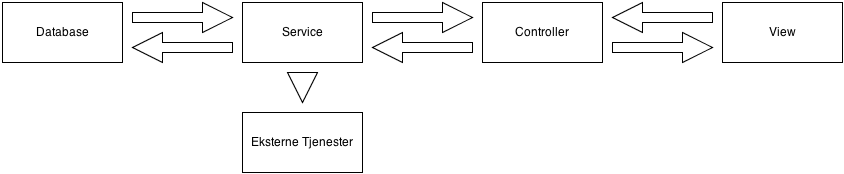
\includegraphics[width=12cm]{webapp-flyt.png}
  \caption{Viser samhandlingen mellom de forskjellige delene i webapplikasjonen}
\end{figure}

\subsubsection{ER modellen}
ER modellen gjennomgikk mange forandringer før vi fikk en modell som “funket”. Modellen var ustabil lenge og vi støtte stadig på problemer som gjorde at vi prøvde nye måter å sette opp modellen på. Til slutt bestemte vi oss på å lage en begrenset dynamisk system, det vil si vi lagde modellen med en begrenset og statisk trestruktur. Med dette la vi “eieransvaret” for relasjonene til hovedlagene (fremsiden, studier, kurs) og under disse, fragmentene som igjen eide de nederste objektene (video, dokumenter, artikler osv). \newline
Vi traff på “orphan” problematikken i relasjonsdatabasen. Dette problemet fremkommer i many to many tilkoblinger og oppstår når et av objektene med relasjoner blir slettet. Problemstillingen er hva som skal skje med det gjenværende objektet. For eksempel: et fragment er knyttet til en video. En administrator sletter videoen. Nå er videoen slettet, men fragmentet har fortsatt en relasjon til videoen selv om den ikke eksisterer lenger. Dette gjorde at applikasjonen fikk feilmelding hver gang den prøvde å laste inn objektet. Vi fikset dette med å legge til “(cascade = CascadeType.ALL)” til “@ManyToMany” deklarasjonen i fragmentet for video feltet slik at det ble slik.

\begin{lstlisting}[language=Java, frame=single]
@ManyToMany(cascade = CascadeType.ALL)
List<Video> videos;
\end{lstlisting}
Dette gjør at fragmentet i dette tilfelle blir “eieren” av relasjonen. \newline
\newline
Vi hadde også problemer med “infinite loops” i JSON tjenestene. For eksempel et fragment inneholder en referanse til en video som inneholder en referanse til fragmentet som inneholder en referanse til video osv. Dette fikset vi med å bruke “@XmlTransient” taggen i get metodene for referansen til en av de to objektene med konflikter, i dette tilfellet video.

\begin{lstlisting}[language=Java, frame=single]
@XmlTransient
public List<Fragment> getFragments() {
    return fragments;
}
\end{lstlisting}
Dette gjorde at når JSONen for fragmentet blir skrevet inneholder fragmentet en referanse til video, men video viser ikke sin referanse til fragmentet, dette løste problemet.\newline
\newline
I løpet av dette prosjektet lærte vi mye om relasjonsdatabaser og problematikken rundt disse, spesielt om man prøver å lage et komplekst fleksibelt system.

\subsubsection{Serversikkerhet}

Da prosjektet startet ble det satt opp en webserver som skulle bli brukt for å publisere webserveren under utviklingen. Denne serveren ble ikke høyt prioritert, og hadde derfor kun grunnleggende sikkerhet. \newline
I perioden 30. mars til 2. april(påske) klarte en hacker gruppe å bryte seg inn på denne serveren. Dette ble oppdaget den 3. april. Gruppen hadde klart å bryte seg inn over SSH ved å gjette seg frem til riktig passord. Dette ble mest sansynlig gjort ved å automatisk teste vanlige passord fra den engelske ordlisten. Hackerene la igjen navnet(Cracker clan) og IP adressen sin(82.137.13.148) i loggen, men disse sporene ledet ikke til noe nyttig informasjon. \newline
Hva hackerene gjorde på serveren kom ikke helt klart frem, så det ble bestemt at serveren skulle slettes fra clusteret, og det skulle opprettes en ny. \newline
Den nye serveren er satt opp med passord som ikke finnes i noen ordliste, og man er begrenset til 3 forsøk og begrenset tid for å logge inn. Dette gjør at datakraften og tiden nødvendig for å bryte seg inn er så høy at det sansynligvis ikke er verdt bryet. Selv om hackerene klarer å gjette 1012 ganger i sekundet, vil det fremdeles ta ca. 1,6 år før de finner rett passord.

\subsubsection{Manglende eller ikke-implementert mulig funksjonalitet}

Denne delen handler om funksjonalitet i både Web- og mobil-applikasjon som ikke er implementert men enten burde eller kunne ha vært inkludert. Av disse to er manglene viktigst, m.a.o funksjonalitet som ikke er ferdigstilt og må anses som mangler. \newline
\newline
I web-applikasjons ble et system for oppretting og håndtering studieløp implementert, men en mangel kan være at studieløpet ikke deles opp i årsklasser. \newline
\newline
Felles for web-og mobil-applikasjon eksisterer det ikke noe reelt brukersystem. For å få full nytte av annen eksisterende funksjonalitet som f.eks Quiz eller Fronter-delen er et slikt system nødvendig.\newline
\newline
En av de opplagte funksjonen som vi ikke rakk å implementere er styring av rekkefølgen av fragmentene på mobilapplikasjonen. Fragmentene er i denne versjonen av systemet vist i rekkefølgen til fragmentets interne ID. Vi ønsket å lage enten et “numerisk” rekkefølge system der brukeren manuelt legger inn rekkefølgen, eller et automatisk system der fragmentene følger en statisk prioritetsliste. 

\subsubsection{Gjenværende bugs}

\begin{itemize}
\item Hver gang webapplikasjonen blir publisert på nytt slettes alle fragmentene på fremsiden. - lav prioritet, om system faktisk blir satt i bruk vil man ikke å publisere webapplikasjonen på nytt ofte.
\item Bug med lagring av tema, oppgaver, obligatoriske innleveringer og eksamener på fagnivået - lav prioritet siden informasjonen godt kan lagres som en artikkel. Burde gjøres en vurdering om disse feltene er nødvendige, eller om artikkelfunksjonen er god nok til å erstatte de helt.
\end{itemize}

\subsubsection{Fremtid}

Ikonene for alle fragmentene med unntak av TimeEdit, Fronter og BibSys er hentet fra Internett og kan være rettighetsbeskyttet. Denne grafikken burde byttes ut før mobilapplikasjonen allmenn distribueres. En grafiker burde leies inn for å redesigne utseende til mobilapplikasjonen og lage nye ikoner.

\newpage

\end{document}